\scanpage{13}
% Consolidated scan013; root crop decisions and exact source maps accompany this page.
% Full-scan coordinate positions use the integrated reader-B frame.
% archive sheet number: 12
\figure{\resizebox{\linewidth}{!}{%
\begin{tikzpicture}[x=.01cm,y=-.01cm,line cap=round,line join=round,
  every node/.style={inner sep=0pt,font=\fontsize{12}{14}\selectfont}]
\useasboundingbox (20,18) rectangle (2354,1668);
% assembly group rule-h01; root entry 01–10
\draw[black!50,line width=\dimexpr .14pt*200/127\relax] (28,123)--(800,124)--(1570,127)--(2348,129);
% assembly group rule-h02; root entry 01–10
\draw[black!50,line width=\dimexpr .14pt*200/127\relax] (27,209)--(802,210)--(1572,211)--(2295,212);
% assembly group rule-h03; root entry 01–10
\node[anchor=base west,inner sep=0pt,outer sep=0pt] at (30,286) {\unsure{\begin{tikzpicture}[baseline={(0,0)},x=.01cm,y=-.01cm,line cap=round,line join=round]
\useasboundingbox (0,0) rectangle (2310,6);
\begin{pgfinterruptboundingbox}
\begin{scope}[shift={(-30,-286)},draw=black,fill=black]
\draw[black!12,line width=\dimexpr .12pt*200/127\relax] (30,286)--(620,288) (1134,287)--(2340,292);
\end{scope}
\end{pgfinterruptboundingbox}
\end{tikzpicture}}};
% assembly group rule-h04; root entry 01–10
\draw[black!48,line width=\dimexpr .14pt*200/127\relax] (24,555)--(783,553)--(1575,556)--(2343,562);
% assembly group rule-h05; root entry 01–10
\draw[black!45,line width=\dimexpr .14pt*200/127\relax] (27,638)--(788,640)--(1571,645)--(2346,648);
% assembly group rule-h06; root entry 01–10
\draw[black!50,line width=\dimexpr .14pt*200/127\relax] (26,752)--(790,754)--(1570,756)--(2340,762);
% assembly group rule-h07; root entry 01–10
\draw[black!45,line width=\dimexpr .14pt*200/127\relax] (23,842)--(788,840)--(1570,841)--(2307,847);
% assembly group rule-h08; root entry 01–10
\node[anchor=base west,inner sep=0pt,outer sep=0pt] at (23,928) {\unsure{\begin{tikzpicture}[baseline={(0,0)},x=.01cm,y=-.01cm,line cap=round,line join=round]
\useasboundingbox (0,0) rectangle (2315,6);
\begin{pgfinterruptboundingbox}
\begin{scope}[shift={(-23,-928)},draw=black,fill=black]
\draw[black!15,line width=\dimexpr .11pt*200/127\relax] (23,932)--(395,934) (792,929)--(1190,931) (1568,928)--(2338,932);
\end{scope}
\end{pgfinterruptboundingbox}
\end{tikzpicture}}};
% assembly group rule-h09; root entry 01–10
\draw[line width=\dimexpr .18pt*200/127\relax] (21,1090)--(790,1090)--(1570,1087)--(2348,1094);
% assembly group rule-h10; root entry 01–10
\draw[black!48,line width=\dimexpr .14pt*200/127\relax] (23,1204)--(788,1206)--(1570,1204)--(2342,1209);
% assembly group rule-h11; root entry 01–10
\draw[black!48,line width=\dimexpr .14pt*200/127\relax] (22,1298)--(791,1295)--(1570,1297)--(2341,1306);
% assembly group rule-h12; root entry 01–10
\draw[black!45,line width=\dimexpr .14pt*200/127\relax] (26,1564)--(789,1556)--(1570,1560)--(2340,1575);
% assembly group rule-verticals; root entry 01–10
\node[anchor=base west,inner sep=0pt,outer sep=0pt] at (391,195) {\unsure{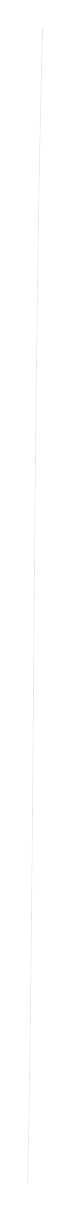
\begin{tikzpicture}[baseline={(0,0)},x=.01cm,y=-.01cm,line cap=round,line join=round]
\useasboundingbox (0,0) rectangle (19,1469);
\begin{pgfinterruptboundingbox}
\begin{scope}[shift={(-391,-195)},draw=black,fill=black]
\draw[black!12,line width=\dimexpr .12pt*200/127\relax] (410,195)..controls (398,620) and (400,1210)..(391,1664);
\end{scope}
\end{pgfinterruptboundingbox}
\end{tikzpicture}}};
\node[anchor=base west,inner sep=0pt,outer sep=0pt] at (1565,23) {\unsure{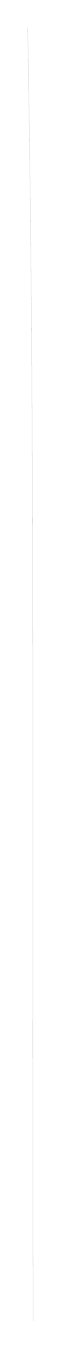
\begin{tikzpicture}[baseline={(0,0)},x=.01cm,y=-.01cm,line cap=round,line join=round]
\useasboundingbox (0,0) rectangle (10,1643);
\begin{pgfinterruptboundingbox}
\begin{scope}[shift={(-1565,-23)},draw=black,fill=black]
\draw[black!12,line width=\dimexpr .12pt*200/127\relax] (1565,23)..controls (1575,561) and (1570,1118)..(1572,1666);
\end{scope}
\end{pgfinterruptboundingbox}
\end{tikzpicture}}};
\node[anchor=base west,inner sep=0pt,outer sep=0pt] at (790,207) {\unsure{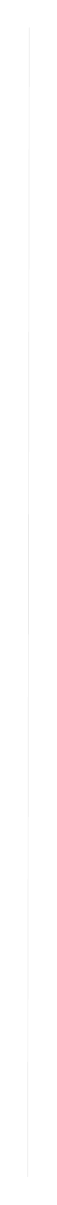
\begin{tikzpicture}[baseline={(0,0)},x=.01cm,y=-.01cm,line cap=round,line join=round]
\useasboundingbox (0,0) rectangle (2,1460);
\begin{pgfinterruptboundingbox}
\begin{scope}[shift={(-790,-207)},draw=black,fill=black]
\draw[black!8,line width=.24pt] (792,207)--(790,1667);
\end{scope}
\end{pgfinterruptboundingbox}
\end{tikzpicture}|{}}};
\node[anchor=base west,inner sep=0pt,outer sep=0pt] at (1184,207) {\unsure{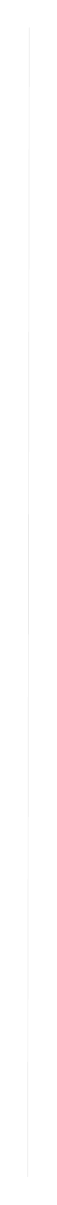
\begin{tikzpicture}[baseline={(0,0)},x=.01cm,y=-.01cm,line cap=round,line join=round]
\useasboundingbox (0,0) rectangle (2,1460);
\begin{pgfinterruptboundingbox}
\begin{scope}[shift={(-1184,-207)},draw=black,fill=black]
\draw[black!8,line width=.24pt] (1186,207)--(1184,1667);
\end{scope}
\end{pgfinterruptboundingbox}
\end{tikzpicture}|{}}};
\node[anchor=base west,inner sep=0pt,outer sep=0pt] at (1967,207) {\unsure{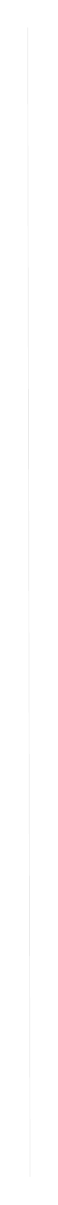
\begin{tikzpicture}[baseline={(0,0)},x=.01cm,y=-.01cm,line cap=round,line join=round]
\useasboundingbox (0,0) rectangle (3,1460);
\begin{pgfinterruptboundingbox}
\begin{scope}[shift={(-1967,-207)},draw=black,fill=black]
\draw[black!8,line width=.24pt] (1967,207)--(1970,1667);
\end{scope}
\end{pgfinterruptboundingbox}
\end{tikzpicture}|{}}};
% assembly group rule-lower-thickening; root entry 32
\node[anchor=base west,inner sep=0pt,outer sep=0pt] at (2221,1300) {\unsure{\begin{tikzpicture}[baseline={(0,0)},x=.01cm,y=-.01cm,line cap=round,line join=round]
\useasboundingbox (0,0) rectangle (14,5);
\begin{pgfinterruptboundingbox}
\begin{scope}[shift={(-2221,-1300)},draw=black,fill=black]
\fill (2221,1304)..controls (2226,1300) and (2231,1302)..(2235,1305)--cycle;
\end{scope}
\end{pgfinterruptboundingbox}
\end{tikzpicture}}};
% assembly group rule-live-thickening; root entry 39
\node[anchor=base west,inner sep=0pt,outer sep=0pt] at (2308,1088) {\unsure{\begin{tikzpicture}[baseline={(0,0)},x=.01cm,y=-.01cm,line cap=round,line join=round]
\useasboundingbox (0,0) rectangle (13,5);
\begin{pgfinterruptboundingbox}
\begin{scope}[shift={(-2308,-1088)},draw=black,fill=black]
\fill (2308,1090)..controls (2314,1088) and (2319,1090)..(2321,1092)--(2311,1093)--cycle;
\end{scope}
\end{pgfinterruptboundingbox}
\end{tikzpicture}}};
% assembly group title1-residuals; root entry 12
\node[anchor=base west,inner sep=0pt,outer sep=0pt] at (137,749) {\unsure{\begin{tikzpicture}[baseline={(0,0)},x=.01cm,y=-.01cm,line cap=round,line join=round]
\useasboundingbox (0,0) rectangle (155,88);
\begin{pgfinterruptboundingbox}
\begin{scope}[shift={(-137,-749)},draw=black,fill=black]
\draw[black!18,line width=\dimexpr .18pt*200/127\relax] (137,749)--(141,790)--(149,837) (160,749)--(164,792)--(168,823) (208,789)--(214,829) (243,795)--(248,834) (287,796)--(292,835);
\end{scope}
\end{pgfinterruptboundingbox}
\end{tikzpicture}}};
% assembly group heading1; reader-B typography; exact common source content
\node[anchor=base,font=\fontsize{14}{16}\selectfont] (heading1) at (215,126) {Notes};
% assembly group notes-number1; reader-B typography; exact common source content
\node[anchor=base,font=\fontsize{14}{16}\selectfont] (notes-number1) at (215,207) {1};
% assembly group heading2; reader-B typography; exact common source content
\node[anchor=base,font=\fontsize{14}{16}\selectfont] (heading2) at (593,126) {Notes};
% assembly group notes-number2; reader-B typography; exact common source content
\node[anchor=base,font=\fontsize{14}{16}\selectfont] (notes-number2) at (593,207) {5};
% assembly group heading3; reader-B typography; exact common source content
\node[anchor=base,font=\fontsize{14}{16}\selectfont] (heading3) at (986,126) {Notes};
% assembly group notes-number3; reader-B typography; exact common source content
\node[anchor=base,font=\fontsize{14}{16}\selectfont] (notes-number3) at (986,207) {7};
% assembly group heading4; reader-B typography; exact common source content
\node[anchor=base,font=\fontsize{14}{16}\selectfont] (heading4) at (1357,126) {Notes};
% assembly group notes-number4; reader-B typography; exact common source content
\node[anchor=base,font=\fontsize{14}{16}\selectfont] (notes-number4) at (1357,207) {15};
% assembly group heading5; reader-B typography; exact common source content
\node[anchor=base,font=\fontsize{14}{16}\selectfont] (heading5) at (1746,126) {Notes};
% assembly group notes-number5; reader-B typography; exact common source content
\node[anchor=base,font=\fontsize{14}{16}\selectfont] (notes-number5) at (1746,207) {20};
% assembly group heading6; reader-B typography; exact common source content
\node[anchor=base,font=\fontsize{14}{16}\selectfont] (heading6) at (2153,126) {Notes};
% assembly group notes-number6; reader-B typography; exact common source content
\node[anchor=base,font=\fontsize{14}{16}\selectfont] (notes-number6) at (2153,207) {23};
% assembly group cancelled-date; root entry 24
\node[anchor=base west,inner sep=\dimexpr 0pt*200/127\relax,font=\scriptsize] at (84,293) {\resizebox{\dimexpr 1.53035cm*200/127\relax}{!}{\rlap{A (1976/77)}\phantom{\deleted{A (1976/77)}}}};
% assembly group cancelled-date-hatching; root entry 24
\draw[black!72,line width=\dimexpr .27pt*200/127\relax] (94,290)--(112,251);
\draw[black!72,line width=\dimexpr .27pt*200/127\relax] (109,290)--(130,248);
\draw[black!72,line width=\dimexpr .27pt*200/127\relax] (124,290)--(145,246);
\draw[black!72,line width=\dimexpr .27pt*200/127\relax] (139,290)--(160,251);
\draw[black!72,line width=\dimexpr .27pt*200/127\relax] (154,291)--(174,254);
\draw[black!72,line width=\dimexpr .27pt*200/127\relax] (167,293)--(188,250);
\draw[black!72,line width=\dimexpr .27pt*200/127\relax] (181,296)--(202,247);
\draw[black!72,line width=\dimexpr .27pt*200/127\relax] (196,297)--(216,246);
\draw[black!72,line width=\dimexpr .27pt*200/127\relax] (210,298)--(230,243);
\draw[black!72,line width=\dimexpr .27pt*200/127\relax] (224,299)--(242,241);
\draw[black!72,line width=\dimexpr .27pt*200/127\relax] (239,299)..controls (245,301) and (249,280)..(259,239);
\draw[black!72,line width=\dimexpr .27pt*200/127\relax] (255,302)..controls (262,306) and (270,276)..(276,240);
\draw[black!72,line width=\dimexpr .27pt*200/127\relax] (274,298)--(293,249);
\draw[black!72,line width=\dimexpr .27pt*200/127\relax] (290,302)..controls (296,305) and (305,276)..(313,251);
% assembly group old-A; root entry 11
\node[anchor=base west,inner sep=\dimexpr 0pt*200/127\relax,font=\scriptsize,text=black!38] at (187,579) {\resizebox{\dimexpr 0.26670cm*200/127\relax}{!}{\unsure{\rlap{A}\phantom{\deleted{A}}|A}}};
% assembly group G-old-A-curves; root entry 11
\node[anchor=base west,inner sep=0pt,outer sep=0pt] at (173,555) {\unsure{\begin{tikzpicture}[baseline={(0,0)},x=.01cm,y=-.01cm,line cap=round,line join=round]
\useasboundingbox (0,0) rectangle (61,30);
\begin{pgfinterruptboundingbox}
\begin{scope}[shift={(-173,-555)},draw=black,fill=black]
\draw[black!28,line width=\dimexpr .18pt*200/127\relax] (178,555)..controls (173,565) and (180,579)..(186,585);
\draw[black!28,line width=\dimexpr .18pt*200/127\relax] (230,555)..controls (234,567) and (234,578)..(230,585);
\end{scope}
\end{pgfinterruptboundingbox}
\end{tikzpicture}}};
% assembly group letter1; reader-B typography; exact common source content
\node[anchor=base,font=\fontsize{20}{22}\selectfont] (letter1) at (205,557) {A};
% assembly group date1; reader-B typography; exact common source content
\node[anchor=base,font=\fontsize{13}{15}\selectfont] (date1) at (214,641) {(1976/77)};
% assembly group letter2; reader-B typography; exact common source content
\node[anchor=base,font=\fontsize{20}{22}\selectfont] (letter2) at (568,557) {B};
% assembly group date2; reader-B typography; exact common source content
\node[anchor=base,font=\fontsize{13}{15}\selectfont] (date2) at (586,641) {(1978/79)};
% assembly group letter3; reader-B typography; exact common source content
\node[anchor=base,font=\fontsize{20}{22}\selectfont] (letter3) at (977,557) {C};
% assembly group date3; reader-B typography; exact common source content
\node[anchor=base,font=\fontsize{13}{15}\selectfont] (date3) at (982,641) {(1979/80)};
% assembly group letter4; reader-B typography; exact common source content
\node[anchor=base,font=\fontsize{20}{22}\selectfont] (letter4) at (1332,557) {D};
% assembly group date4; reader-B typography; exact common source content
\node[anchor=base,font=\fontsize{13}{15}\selectfont] (date4) at (1335,641) {(1980)};
% assembly group letter5; reader-B typography; exact common source content
\node[anchor=base,font=\fontsize{20}{22}\selectfont] (letter5) at (1732,557) {E};
% assembly group date5; reader-B typography; exact common source content
\node[anchor=base,font=\fontsize{13}{15}\selectfont] (date5) at (1740,641) {(1981)};
% assembly group letter6; reader-B typography; exact common source content
\node[anchor=base,font=\fontsize{20}{22}\selectfont] (letter6) at (2128,557) {E};
% assembly group date6; reader-B typography; exact common source content
\node[anchor=base,font=\fontsize{13}{15}\selectfont] (date6) at (2133,641) {(1981)};
% assembly group margin-core; root entry 25
\draw[line width=\dimexpr .42pt*200/127\relax] (32,414)--(65,414);
\draw[black!65,line width=\dimexpr .25pt*200/127\relax] (48,422)..controls (47,477) and (47,514)..(43,554)..controls (42,597) and (46,631)..(40,664);
\draw[line width=\dimexpr .43pt*200/127\relax] (35,436)--(47,420)--(63,438) (47,420)--(62,423);
\draw[black!35,line width=\dimexpr .18pt*200/127\relax] (47,426)--(38,448);
\draw[line width=\dimexpr .31pt*200/127\relax] (66,496)..controls (48,487) and (55,553)..(57,591)..controls (60,629) and (54,655)..(44,666)..controls (58,673) and (63,676)..(64,708)..controls (65,755) and (64,805)..(66,829)..controls (67,842) and (70,847)..(74,847);
\draw[black!35,line width=\dimexpr .22pt*200/127\relax] (48,500)..controls (48,552) and (43,612)..(41,663)..controls (44,678) and (51,678)..(51,705)..controls (52,753) and (53,809)..(54,845);
\draw[line width=\dimexpr .18pt*200/127\relax] (48,556)..controls (40,565) and (43,586)..(48,604);
\draw[black!65,line width=\dimexpr .23pt*200/127\relax] (120,555)--(119,578)..controls (119,588) and (117,592)..(111,596)..controls (118,600) and (120,610)..(122,638);
\draw[line width=\dimexpr .24pt*200/127\relax] (114,568)--(119,578)--(124,571) (111,619)--(118,608)--(126,619);
\draw[black!32,line width=\dimexpr .17pt*200/127\relax] (112,554)--(112,563) (109,559)--(112,563)--(115,559);
% assembly group upper-question; root entry 25
\node[anchor=base,font=\fontsize{17}{19}\selectfont] (upper-question) at (86,616) {?};
% assembly group G-margin-point; root entry 25
\node[anchor=base west,inner sep=0pt,outer sep=0pt] at (46,402) {\unsure{\begin{tikzpicture}[baseline={(0,0)},x=.01cm,y=-.01cm,line cap=round,line join=round]
\useasboundingbox (0,0) rectangle (2,4);
\begin{pgfinterruptboundingbox}
\begin{scope}[shift={(-46,-402)},draw=black,fill=black]
\fill[black!40] (47,404) ellipse[x radius=.9,y radius=1.8];
\end{scope}
\end{pgfinterruptboundingbox}
\end{tikzpicture}}};
% assembly group G-bent-upper; root entry 26
\draw[line width=\dimexpr .31pt*200/127\relax] (254,667)--(319,667)--(318,644) (312,650)--(318,644)--(324,653);
% assembly group G-bent-upper-arch; root entry 26
\node[anchor=base west,inner sep=0pt,outer sep=0pt] at (257,657) {\unsure{\begin{tikzpicture}[baseline={(0,0)},x=.01cm,y=-.01cm,line cap=round,line join=round]
\useasboundingbox (0,0) rectangle (21,8);
\begin{pgfinterruptboundingbox}
\begin{scope}[shift={(-257,-657)},draw=black,fill=black]
\draw[black!38,line width=\dimexpr .18pt*200/127\relax] (257,665)..controls (265,662) and (273,657)..(278,661);
\end{scope}
\end{pgfinterruptboundingbox}
\end{tikzpicture}}};
% assembly group G-bent-upper-dash; root entry 26
\node[anchor=base west,inner sep=0pt,outer sep=0pt] at (307,652) {\unsure{\begin{tikzpicture}[baseline={(0,0)},x=.01cm,y=-.01cm,line cap=round,line join=round]
\useasboundingbox (0,0) rectangle (4,2);
\begin{pgfinterruptboundingbox}
\begin{scope}[shift={(-307,-652)},draw=black,fill=black]
\draw[black!63,line width=\dimexpr .21pt*200/127\relax] (307,652)--(311,654);
\end{scope}
\end{pgfinterruptboundingbox}
\end{tikzpicture}}};
% assembly group G-bent-upper-dot; root entry 26
\node[anchor=base west,inner sep=0pt,outer sep=0pt] at (303,671) {\unsure{\begin{tikzpicture}[baseline={(0,0)},x=.01cm,y=-.01cm,line cap=round,line join=round]
\useasboundingbox (0,0) rectangle (2,4);
\begin{pgfinterruptboundingbox}
\begin{scope}[shift={(-303,-671)},draw=black,fill=black]
\fill[black!58] (304,673) ellipse[x radius=.8,y radius=1.3];
\end{scope}
\end{pgfinterruptboundingbox}
\end{tikzpicture}}};
% assembly group G-bent-lower; root entry 26
\draw[line width=\dimexpr .34pt*200/127\relax] (255,701)..controls (267,707) and (293,706)..(308,709)--(325,711)--(325,735) (318,728)--(325,736)--(332,731);
% assembly group G-bent-lower-retrace; root entry 26
\draw[line width=\dimexpr .25pt*200/127\relax] (254,713)--(277,713)--(306,710)--(317,710);
% assembly group G-date-hook; root entry 27
\node[anchor=base west,inner sep=0pt,outer sep=0pt] at (401,616) {\unsure{\begin{tikzpicture}[baseline={(0,0)},x=.01cm,y=-.01cm,line cap=round,line join=round]
\useasboundingbox (0,0) rectangle (17,25);
\begin{pgfinterruptboundingbox}
\draw[black!55,line width=.35pt] (11,3)..controls (11,11) and (8,16)..(5,20);
\draw[black!25,line width=.25pt] (5,21)--(4,24);
\begin{scope}[shift={(-401,-616)}]
\draw[black!70,line width=.50pt] (404,639)--(417,640);
\end{scope}
\end{pgfinterruptboundingbox}
\end{tikzpicture}}};
% assembly group title1a; reader-B typography; exact common source content
\node[anchor=base,font=\fontsize{14}{16}\selectfont] (title1a) at (218,752) {Découverte};
% assembly group title1b; reader-B typography; exact common source content
\node[anchor=base,font=\fontsize{11}{13}\selectfont] (title1b) at (201,786) {de la};
% assembly group title1c; root entry 12
\node[anchor=base,font=\fontsize{14}{16}\selectfont] (title1c) at (236,838) {Méditation};
% assembly group title2a; reader-B typography; exact common source content
\node[anchor=base,font=\fontsize{14}{16}\selectfont] (title2a) at (586,753) {Réveil};
% assembly group G-Reveil-diagonal; root entry 13
\node[anchor=base west,inner sep=0pt,outer sep=0pt] at (500,694) {\unsure{\begin{tikzpicture}[baseline={(0,0)},x=.01cm,y=-.01cm,line cap=round,line join=round]
\useasboundingbox (0,0) rectangle (58,55);
\begin{pgfinterruptboundingbox}
\begin{scope}[shift={(-500,-694)},draw=black,fill=black]
\fill (501,694)..controls (505,694) and (509,697)..(509,703)..controls (505,703) and (502,700)..(500,697)--cycle;
\draw[black!65,line width=\dimexpr .19pt*200/127\relax] (513,706)--(517,710);
\draw[black!26,line width=\dimexpr .17pt*200/127\relax] (518,711)--(529,721);
\fill[black!35] (533,728)--(537,730)--(541,729)--(539,734)--(536,734)--cycle;
\draw[black!55,line width=\dimexpr .18pt*200/127\relax] (549,739)--(552,742) (554,744)--(558,749);
\end{scope}
\end{pgfinterruptboundingbox}
\end{tikzpicture}}};
% assembly group title2b; reader-B typography; exact common source content
\node[anchor=base,font=\fontsize{11}{13}\selectfont] (title2b) at (576,790) {en};
% assembly group old-C-Ca; root entry 13
\node[anchor=base,font=\fontsize{14}{16}\selectfont,text=black!65] (old-C-Ca) at (525,837) {\rlap{\unsure{C|Ca}}\phantom{\deleted{\unsure{C|Ca}}}};
% assembly group title2c; reader-B typography; exact common source content
\node[anchor=base,font=\fontsize{14}{16}\selectfont] (title2c) at (615,839) {Cascades};
% assembly group title3a; reader-B typography; exact common source content
\node[anchor=base,font=\fontsize{14}{16}\selectfont] (title3a) at (966,752) {Die Eltern};
% assembly group title3b; reader-B typography; exact common source content
\node[anchor=base,font=\fontsize{13}{15}\selectfont] (title3b) at (970,839) {(Les parents)};
% assembly group title4a; reader-B typography; exact common source content
\node[anchor=base,font=\fontsize{14}{16}\selectfont] (title4a) at (1348,752) {Das Kind};
% assembly group title4b; reader-B typography; exact common source content
\node[anchor=base,font=\fontsize{13}{15}\selectfont] (title4b) at (1350,839) {(L'enfant)};
% assembly group title5a; reader-B typography; exact common source content
\node[anchor=base,font=\fontsize{14}{16}\selectfont] (title5a) at (1754,754) {Der Baumeister};
% assembly group title5b; reader-B typography; exact common source content
\node[anchor=base,font=\fontsize{13}{15}\selectfont] (title5b) at (1757,840) {(Le Bâtisseur)};
% assembly group title6a; reader-B typography; exact common source content
\node[anchor=base,font=\fontsize{14}{16}\selectfont] (title6a) at (2153,759) {Le Bâtisseur};
% assembly group G-Baumeister-upper-gray; root entry 28
\node[anchor=base west,inner sep=0pt,outer sep=0pt] at (1789,697) {\unsure{\begin{tikzpicture}[baseline={(0,0)},x=.01cm,y=-.01cm,line cap=round,line join=round]
\useasboundingbox (0,0) rectangle (10,12);
\begin{pgfinterruptboundingbox}
\fill[black!40] (5,5) circle [radius=0.01500cm];
\end{pgfinterruptboundingbox}
\end{tikzpicture}}};
% assembly group G-Baumeister-upper-black; root entry 28
\node[anchor=base west,inner sep=0pt,outer sep=0pt] at (1850,695) {\unsure{\begin{tikzpicture}[baseline={(0,0)},x=.01cm,y=-.01cm,line cap=round,line join=round]
\useasboundingbox (0,0) rectangle (14,14);
\begin{pgfinterruptboundingbox}
\fill[black] (4,9)--(6,4)--(10,4)--(9,9)--(6,11)--cycle;
\draw[black!25,line width=.25pt] (10,4)--(12,3);
\end{pgfinterruptboundingbox}
\end{tikzpicture}}};
% assembly group G-Baumeister-left-gray; root entry 28
\node[anchor=base west,inner sep=0pt,outer sep=0pt] at (1689,730) {\unsure{\begin{tikzpicture}[baseline={(0,0)},x=.01cm,y=-.01cm,line cap=round,line join=round]
\useasboundingbox (0,0) rectangle (9,10);
\begin{pgfinterruptboundingbox}
\fill[black!35] (4,4) ellipse [x radius=0.01000cm,y radius=0.01800cm];
\end{pgfinterruptboundingbox}
\end{tikzpicture}}};
% assembly group G-Baumeister-right-gray; root entry 28
\node[anchor=base west,inner sep=0pt,outer sep=0pt] at (1897,736) {\unsure{\begin{tikzpicture}[baseline={(0,0)},x=.01cm,y=-.01cm,line cap=round,line join=round]
\useasboundingbox (0,0) rectangle (12,13);
\begin{pgfinterruptboundingbox}
\draw[black!25,line width=.3pt] (5,4)--(5,8);
\end{pgfinterruptboundingbox}
\end{tikzpicture}}};
% assembly group cancel-A; root entry 14
\node[anchor=base,font=\fontsize{11}{13}\selectfont] (cancel-A) at (205,932) {\rlap{$(\unsure{\mathrm i})$}\phantom{\deleted{$(\unsure{\mathrm i})$}}};
% assembly group hatch-A; root entry 14
\draw[line width=\dimexpr .30pt*200/127\relax] (181,925)--(196,894);
\draw[line width=\dimexpr .30pt*200/127\relax] (185,929)--(201,904);
\draw[line width=\dimexpr .30pt*200/127\relax] (190,933)--(209,905);
\draw[line width=\dimexpr .30pt*200/127\relax] (196,931)--(218,909);
\draw[line width=\dimexpr .30pt*200/127\relax] (203,933)--(224,917);
% assembly group cancel-B; root entry 15
\node[anchor=base west,inner sep=\dimexpr 0pt*200/127\relax,font=\scriptsize] at (560,933) {\resizebox{\dimexpr 0.36830cm*200/127\relax}{!}{\rlap{(ii)}\phantom{\deleted{(ii)}}}};
% assembly group hatch-B; root entry 15
\draw[line width=\dimexpr .30pt*200/127\relax] (557,930)--(585,897);
\draw[line width=\dimexpr .30pt*200/127\relax] (565,929)--(600,899);
\draw[line width=\dimexpr .30pt*200/127\relax] (576,931)--(607,906);
\draw[line width=\dimexpr .30pt*200/127\relax] (580,933)--(615,916);
% assembly group cancel-C; root entry 16
\node[anchor=base,font=\fontsize{11}{13}\selectfont] (cancel-C) at (975,932) {\rlap{$(\unsure{\mathrm i|\mathrm{ii}})$}\phantom{\deleted{$(\unsure{\mathrm i|\mathrm{ii}})$}}};
% assembly group hatch-C; root entry 16
\draw[line width=.6pt] (949,922)--(975,897);
\draw[line width=.6pt] (955,929)--(983,904);
\draw[line width=.6pt] (971,931)--(994,913);
\draw[line width=.6pt] (973,932)--(997,926);
% assembly group cancel-D; root entry 17
\node[anchor=base west,inner sep=\dimexpr 0pt*200/127\relax,font=\scriptsize] at (1319,926) {\resizebox{\dimexpr 0.28575cm*200/127\relax}{!}{\rlap{(i)}\phantom{\deleted{(i)}}}};
% assembly group hatch-D; root entry 17
\draw[line width=\dimexpr .30pt*200/127\relax] (1317,921)--(1336,904);
\draw[line width=\dimexpr .30pt*200/127\relax] (1320,921)--(1343,907);
\draw[line width=\dimexpr .30pt*200/127\relax] (1325,923)--(1351,911);
\draw[line width=\dimexpr .30pt*200/127\relax] (1330,924)--(1362,916);
% assembly group cancel-E20; root entry 18
\node[anchor=base west,inner sep=\dimexpr 0pt*200/127\relax,font=\scriptsize] at (1722,927) {\resizebox{\dimexpr 0.29845cm*200/127\relax}{!}{\rlap{(\unsure{i|ii})}\phantom{\deleted{(\unsure{i|ii})}}}};
% assembly group hatch-E20; root entry 18
\draw[line width=\dimexpr .30pt*200/127\relax] (1718,920)--(1735,903);
\draw[line width=\dimexpr .30pt*200/127\relax] (1722,919)--(1743,905);
\draw[line width=\dimexpr .30pt*200/127\relax] (1728,921)--(1756,906);
\draw[line width=\dimexpr .30pt*200/127\relax] (1733,925)--(1766,916);
% assembly group cancel-E23; root entry 19
\node[anchor=base,font=\fontsize{11}{13}\selectfont] (cancel-E23) at (2161,932) {\rlap{$(\unsure{\mathrm{iii}|\mathrm{iv}})$}\phantom{\deleted{$(\unsure{\mathrm{iii}|\mathrm{iv}})$}}};
% assembly group hatch-E23; root entry 19
\draw[line width=.6pt] (2128,918)--(2144,903);
\draw[line width=.6pt] (2130,920)--(2157,904);
\draw[line width=.6pt] (2146,923)--(2172,909);
\draw[line width=.6pt] (2148,924)--(2185,913);
% assembly group cancel-C-terminal-hook; root entry 16
\draw[line width=.45pt] (993,926)..controls (998,925) and (1000,930)..(1000,934);
% assembly group cancel-E23-terminal-hook; root entry 19
\draw[line width=.5pt] (2190,925)..controls (2196,923) and (2197,930)..(2201,934);
% assembly group G-cancel-C-gray-point; root entry 16
\node[anchor=base west,inner sep=0pt,outer sep=0pt] at (938,892) {\unsure{\begin{tikzpicture}[baseline={(0,0)},x=.01cm,y=-.01cm,line cap=round,line join=round]
\useasboundingbox (0,0) rectangle (12,12);
\begin{pgfinterruptboundingbox}
\fill[black!35] (3,3)--(7,2)--(8,6)--(4,7)--cycle;
\end{pgfinterruptboundingbox}
\end{tikzpicture}}};
% assembly group lower-question; root entry 14
\node[anchor=base,font=\fontsize{15}{17}\selectfont,text=black!40] (lower-question) at (132,975) {?};
% assembly group G-lower-A-arrow; root entry 14
\node[anchor=base west,inner sep=0pt,outer sep=0pt] at (149,910) {\unsure{\begin{tikzpicture}[baseline={(0,0)},x=.01cm,y=-.01cm,line cap=round,line join=round]
\useasboundingbox (0,0) rectangle (27,91);
\begin{pgfinterruptboundingbox}
\begin{scope}[shift={(-149,-910)},draw=black,fill=black]
\draw[black!25,line width=\dimexpr .18pt*200/127\relax] (176,921)..controls (160,910) and (158,918)..(159,936)--(157,1001) (149,992)--(157,1001)--(165,992);
\end{scope}
\end{pgfinterruptboundingbox}
\end{tikzpicture}}};
% assembly group G-lower-B-arrow; root entry 15
\node[anchor=base west,inner sep=0pt,outer sep=0pt] at (526,984) {\unsure{\begin{tikzpicture}[baseline={(0,0)},x=.01cm,y=-.01cm,line cap=round,line join=round]
\useasboundingbox (0,0) rectangle (16,71);
\begin{pgfinterruptboundingbox}
\begin{scope}[shift={(-526,-984)},draw=black,fill=black]
\draw[draw=black!25,line width=\dimexpr 1.4pt*7227/25400\relax] (526,984)..controls(526,1008)and(526,1023)..(533,1042)--(538,1051);
\draw[draw=black!60,line width=\dimexpr 1.4pt*7227/25400\relax] (529,1047)..controls(533,1051)and(536,1050)..(538,1050)--(542,1055);
\end{scope}
\end{pgfinterruptboundingbox}
\end{tikzpicture}}};
% assembly group old-sub-A; root entry 20
\node[anchor=base west,inner sep=\dimexpr 0pt*200/127\relax,font=\scriptsize,text=black!25] at (168,1121) {\resizebox{\dimexpr 0.25400cm*200/127\relax}{!}{\unsure{\rlap{(i)}\phantom{\deleted{(i)}}|(i)}}};
% assembly group live-sub1; reader-B typography; exact common source content
\node[anchor=base,font=\fontsize{12}{14}\selectfont] (live-sub1) at (187,1090) {(i)};
% assembly group live-sub2; reader-B typography; exact common source content
\node[anchor=base,font=\fontsize{12}{14}\selectfont] (live-sub2) at (582,1090) {(ii)};
% assembly group old-sub-C-left; root entry 21
\node[anchor=base west,inner sep=\dimexpr 0pt*200/127\relax,font=\scriptsize,text=black!32] at (945,1080) {\resizebox{\dimexpr 0.24765cm*200/127\relax}{!}{\unsure{\rlap{\unsure{(i)|(}}\phantom{\deleted{\unsure{(i)|(}}}|\unsure{(i)|(}}}};
% assembly group G-live-C-gray-dot; root entry 21
% G-live-C-gray-dot: source component evidence represented within old-sub-C-left; no separate path.
% assembly group G-live-C-right-curve; root entry 21
% G-live-C-right-curve: source component evidence represented within old-sub-C-left; no separate path.
% assembly group live-sub3; reader-B typography; exact common source content
\node[anchor=base,font=\fontsize{12}{14}\selectfont] (live-sub3) at (964,1090) {(i)};
% assembly group old-sub-D; root entry 22
\node[anchor=base west,inner sep=\dimexpr 0pt*200/127\relax,font=\scriptsize,text=black!45] at (1321,1071) {\resizebox{\dimexpr 0.28575cm*200/127\relax}{!}{\unsure{\rlap{(i)}\phantom{\deleted{(i)}}|(i)}}};
% assembly group live-sub4; reader-B typography; exact common source content
\node[anchor=base,font=\fontsize{12}{14}\selectfont] (live-sub4) at (1346,1090) {(i)};
% assembly group live-sub5; reader-B typography; exact common source content
\node[anchor=base,font=\fontsize{12}{14}\selectfont] (live-sub5) at (1746,1090) {(i)};
% assembly group live-sub6; reader-B typography; exact common source content
\node[anchor=base,font=\fontsize{12}{14}\selectfont] (live-sub6) at (2144,1090) {(iv)};
% assembly group lower-title1; reader-B typography; exact common source content
\node[anchor=base,font=\fontsize{14}{16}\selectfont] (lower-title1) at (185,1204) {Envol};
% assembly group lower-title2; root entry 23
\node[anchor=base,font=\fontsize{12}{14}\selectfont] (lower-title2) at (593,1204) {Vers un plus long Voyage};
% assembly group lower-title3; reader-B typography; exact common source content
\node[anchor=base,font=\fontsize{14}{16}\selectfont] (lower-title3) at (1001,1203) {Bild und Wahrheit};
% assembly group lower-trans3; reader-B typography; exact common source content
\node[anchor=base,font=\fontsize{13}{15}\selectfont] (lower-trans3) at (971,1299) {(Image et Réalité)};
% assembly group lower-title4; reader-B typography; exact common source content
\node[anchor=base,font=\fontsize{15}{17}\selectfont] (lower-title4) at (1344,1204) {Der Wolf};
% assembly group lower-trans4; reader-B typography; exact common source content
\node[anchor=base,font=\fontsize{13}{15}\selectfont] (lower-trans4) at (1351,1300) {(Le Loup)};
% assembly group lower-title5; reader-B typography; exact common source content
\node[anchor=base,font=\fontsize{14}{16}\selectfont] (lower-title5) at (1769,1206) {Spiel- und Sucht};
% assembly group lower-trans5; reader-B typography; exact common source content
\node[anchor=base,font=\fontsize{13}{15}\selectfont] (lower-trans5) at (1763,1301) {(Jeu - et Fringale)};
% assembly group lower-title6; reader-B typography; exact common source content
\node[anchor=base,font=\fontsize{15}{17}\selectfont] (lower-title6) at (2152,1207) {Le ``Maître''};
% assembly group G-long-dot; root entry 23
\node[anchor=base west,inner sep=0pt,outer sep=0pt] at (590,1237) {\unsure{\begin{tikzpicture}[baseline={(0,0)},x=.01cm,y=-.01cm,line cap=round,line join=round]
\useasboundingbox (0,0) rectangle (6,6);
\begin{pgfinterruptboundingbox}
\begin{scope}[shift={(-590,-1237)},draw=black,fill=black]
\fill (590,1240)..controls (592,1237) and (595,1238)..(596,1239)..controls (594,1242) and (591,1243)..(590,1240)--cycle;
\end{scope}
\end{pgfinterruptboundingbox}
\end{tikzpicture}}};
% assembly group G-Jeu-overmark; root entry 29
\node[anchor=base west,inner sep=0pt,outer sep=0pt] at (1612,1255) {\unsure{\begin{tikzpicture}[baseline={(0,0)},x=.01cm,y=-.01cm,line cap=round,line join=round]
\useasboundingbox (0,0) rectangle (12,12);
\begin{pgfinterruptboundingbox}
\fill[black!70] (3,5)--(7,4)--(4,7)--cycle;
\end{pgfinterruptboundingbox}
\end{tikzpicture}}};
% assembly group G-Spiel-lower-spot; root entry 29
\node[anchor=base west,inner sep=0pt,outer sep=0pt] at (1695,1223) {\unsure{\begin{tikzpicture}[baseline={(0,0)},x=.01cm,y=-.01cm,line cap=round,line join=round]
\useasboundingbox (0,0) rectangle (12,13);
\begin{pgfinterruptboundingbox}
\fill[black!25] (5,6) ellipse [x radius=0.01800cm,y radius=0.01500cm];
\end{pgfinterruptboundingbox}
\end{tikzpicture}}};
% assembly group G-A-blank-trace; root entry 30
\node[anchor=base west,inner sep=0pt,outer sep=0pt] at (224,1404) {\unsure{\begin{tikzpicture}[baseline={(0,0)},x=.01cm,y=-.01cm,line cap=round,line join=round]
\useasboundingbox (0,0) rectangle (17,39);
\begin{pgfinterruptboundingbox}
\fill[black!80] (11,4)--(9,8)--(11,11)--(8,14)--(5,13)--(6,8)--cycle;
\fill[black!85] (8,17) ellipse [x radius=0.02000cm,y radius=0.01500cm];
\fill[black!30] (8,25) ellipse [x radius=0.01800cm,y radius=0.01500cm];
\fill[black!30] (4,32) ellipse [x radius=0.01600cm,y radius=0.01400cm];
\fill[black!30] (5,36) ellipse [x radius=0.01600cm,y radius=0.01200cm];
\end{pgfinterruptboundingbox}
\end{tikzpicture}}};
% assembly group G-A-foot-trace; root entry 31
\node[anchor=base west,inner sep=0pt,outer sep=0pt] at (329,1578) {\unsure{\begin{tikzpicture}[baseline={(0,0)},x=.01cm,y=-.01cm,line cap=round,line join=round]
\useasboundingbox (0,0) rectangle (17,37);
\begin{pgfinterruptboundingbox}
\fill[black!25] (12,5) ellipse [x radius=0.02000cm,y radius=0.02000cm];
\fill[black!45] (11,11) circle [radius=0.01500cm];
\fill[black!60] (8,16) ellipse [x radius=0.01500cm,y radius=0.02000cm];
\fill[black!35] (6,22) circle [radius=0.01500cm];
\fill[black!45] (7,26) ellipse [x radius=0.01000cm,y radius=0.01500cm];
\fill[black!50] (4,30) ellipse [x radius=0.02000cm,y radius=0.01300cm];
\fill[black!20] (4,34) ellipse [x radius=0.02000cm,y radius=0.01300cm];
\end{pgfinterruptboundingbox}
\end{tikzpicture}}};
% assembly group G-E23-dash; root entry 32
\node[anchor=base west,inner sep=0pt,outer sep=0pt] at (2252,1343) {\unsure{\begin{tikzpicture}[baseline={(0,0)},x=.01cm,y=-.01cm,line cap=round,line join=round]
\useasboundingbox (0,0) rectangle (16,1);
\begin{pgfinterruptboundingbox}
\begin{scope}[shift={(-2252,-1343)},draw=black,fill=black]
\draw[black!53,line width=\dimexpr .20pt*200/127\relax] (2252,1343)--(2268,1344);
\end{scope}
\end{pgfinterruptboundingbox}
\end{tikzpicture}}};
% assembly group G-E20-blot; root entry 33
\node[anchor=base west,inner sep=0pt,outer sep=0pt] at (1926,1353) {\unsure{\begin{tikzpicture}[baseline={(0,0)},x=.01cm,y=-.01cm,line cap=round,line join=round]
\useasboundingbox (0,0) rectangle (15,19);
\begin{pgfinterruptboundingbox}
\fill[black!25] (6,3)--(9,4)--(11,8)--(9,12)--(6,14)--(3,13)--(5,11)--(4,7)--cycle;
\end{pgfinterruptboundingbox}
\end{tikzpicture}}};
% assembly group G-D-point; root entry 34
\node[anchor=base west,inner sep=0pt,outer sep=0pt] at (1490,1517) {\unsure{\begin{tikzpicture}[baseline={(0,0)},x=.01cm,y=-.01cm,line cap=round,line join=round]
\useasboundingbox (0,0) rectangle (10,11);
\begin{pgfinterruptboundingbox}
\fill[black!70] (4,5) circle [radius=0.01400cm];
\end{pgfinterruptboundingbox}
\end{tikzpicture}}};
% assembly group G-A-edge-slant; root entry 35
\node[anchor=base west,inner sep=0pt,outer sep=0pt] at (368,1013) {\unsure{\begin{tikzpicture}[baseline={(0,0)},x=.01cm,y=-.01cm,line cap=round,line join=round]
\useasboundingbox (0,0) rectangle (24,31);
\begin{pgfinterruptboundingbox}
\fill[black!20] (4,5) ellipse [x radius=0.02500cm,y radius=0.03000cm];
\fill[black!35] (7,11) ellipse [x radius=0.02000cm,y radius=0.02500cm];
\fill[black!35] (10,16) ellipse [x radius=0.02500cm,y radius=0.02000cm];
\fill[black!30] (14,21) ellipse [x radius=0.01500cm,y radius=0.01800cm];
\fill[black!30] (18,25) ellipse [x radius=0.02000cm,y radius=0.01700cm];
\fill[black!25] (12,7) circle [radius=0.01700cm];
\end{pgfinterruptboundingbox}
\end{tikzpicture}}};
% assembly group foot1; reader-B typography; exact common source content
\node[anchor=base,font=\fontsize{15}{17}\selectfont] (foot1) at (203,1564) {M $1976\mathord{*}$};
% assembly group foot2; reader-B typography; exact common source content
\node[anchor=base,font=\fontsize{15}{17}\selectfont] (foot2) at (573,1564) {M 1979};
% assembly group foot3; reader-B typography; exact common source content
\node[anchor=base,font=\fontsize{15}{17}\selectfont] (foot3) at (946,1564) {HS $\mathrm I$};
% assembly group foot4; reader-B typography; exact common source content
\node[anchor=base,font=\fontsize{15}{17}\selectfont] (foot4) at (1312,1564) {Sch $\mathrm I$};
% assembly group foot5; reader-B typography; exact common source content
\node[anchor=base,font=\fontsize{15}{17}\selectfont] (foot5) at (1746,1564) {Sch $\overline{\underline{\mathrm{VI}}}$};
% assembly group foot6; reader-B typography; exact common source content
\node[anchor=base,font=\fontsize{15}{17}\selectfont] (foot6) at (2147,1573) {Sch $\overline{\underline{\mathrm{IX}}}$};
% assembly group G-edge-01; root entry 37
\node[anchor=base west,inner sep=0pt,outer sep=0pt] at (2333,113) {\unsure{\begin{tikzpicture}[baseline={(0,0)},x=.01cm,y=-.01cm,line cap=round,line join=round]
\useasboundingbox (0,0) rectangle (18,19);
\begin{pgfinterruptboundingbox}
\begin{scope}[shift={(-2333,-113)},draw=black,fill=black]
\draw[black!100,line width=\dimexpr .28pt*200/127\relax] (2336,116)--(2349,129) (2334,128)--(2349,129);
\end{scope}
\end{pgfinterruptboundingbox}
\end{tikzpicture}}};
% assembly group G-edge-02; root entry 37
\node[anchor=base west,inner sep=0pt,outer sep=0pt] at (2329,197) {\unsure{\begin{tikzpicture}[baseline={(0,0)},x=.01cm,y=-.01cm,line cap=round,line join=round]
\useasboundingbox (0,0) rectangle (22,15);
\begin{pgfinterruptboundingbox}
\begin{scope}[shift={(-2329,-197)},draw=black,fill=black]
\draw[black!100,line width=\dimexpr .28pt*200/127\relax] (2339,201)--(2349,208) (2332,206)..controls (2339,210) and (2344,207)..(2349,208);
\end{scope}
\end{pgfinterruptboundingbox}
\end{tikzpicture}}};
% assembly group G-edge-03; root entry 37
\node[anchor=base west,inner sep=0pt,outer sep=0pt] at (2327,362) {\unsure{\begin{tikzpicture}[baseline={(0,0)},x=.01cm,y=-.01cm,line cap=round,line join=round]
\useasboundingbox (0,0) rectangle (24,17);
\begin{pgfinterruptboundingbox}
\begin{scope}[shift={(-2327,-362)},draw=black,fill=black]
\draw[black!100,line width=\dimexpr .28pt*200/127\relax] (2330,366)--(2348,375) (2330,373)--(2348,375);
\end{scope}
\end{pgfinterruptboundingbox}
\end{tikzpicture}}};
% assembly group G-edge-04; root entry 37
\node[anchor=base west,inner sep=0pt,outer sep=0pt] at (2326,414) {\unsure{\begin{tikzpicture}[baseline={(0,0)},x=.01cm,y=-.01cm,line cap=round,line join=round]
\useasboundingbox (0,0) rectangle (25,18);
\begin{pgfinterruptboundingbox}
\begin{scope}[shift={(-2326,-414)},draw=black,fill=black]
\draw[black!100,line width=\dimexpr .28pt*200/127\relax] (2329,418)--(2349,426) (2329,427)..controls (2338,430) and (2344,427)..(2349,427);
\end{scope}
\end{pgfinterruptboundingbox}
\end{tikzpicture}}};
% assembly group G-edge-05; root entry 38
\node[anchor=base west,inner sep=0pt,outer sep=0pt] at (2322,548) {\unsure{\begin{tikzpicture}[baseline={(0,0)},x=.01cm,y=-.01cm,line cap=round,line join=round]
\useasboundingbox (0,0) rectangle (25,20);
\begin{pgfinterruptboundingbox}
\begin{scope}[shift={(-2322,-548)},draw=black,fill=black]
\draw[black!100,line width=\dimexpr .28pt*200/127\relax] (2328,552)--(2342,562)--(2343,565) (2325,562)--(2339,562);
\end{scope}
\end{pgfinterruptboundingbox}
\end{tikzpicture}}};
% assembly group G-edge-06; root entry 38
\node[anchor=base west,inner sep=0pt,outer sep=0pt] at (2328,635) {\unsure{\begin{tikzpicture}[baseline={(0,0)},x=.01cm,y=-.01cm,line cap=round,line join=round]
\useasboundingbox (0,0) rectangle (22,19);
\begin{pgfinterruptboundingbox}
\begin{scope}[shift={(-2328,-635)},draw=black,fill=black]
\draw[black!100,line width=\dimexpr .28pt*200/127\relax] (2331,639)--(2347,648) (2336,650)--(2347,648);
\end{scope}
\end{pgfinterruptboundingbox}
\end{tikzpicture}}};
% assembly group G-edge-07; root entry 39
\node[anchor=base west,inner sep=0pt,outer sep=0pt] at (2332,962) {\unsure{\begin{tikzpicture}[baseline={(0,0)},x=.01cm,y=-.01cm,line cap=round,line join=round]
\useasboundingbox (0,0) rectangle (19,19);
\begin{pgfinterruptboundingbox}
\begin{scope}[shift={(-2332,-962)},draw=black,fill=black]
\draw[black!45,line width=\dimexpr .28pt*200/127\relax] (2338,965)--(2346,975) (2335,977)--(2345,977)--(2348,973);
\end{scope}
\end{pgfinterruptboundingbox}
\end{tikzpicture}}};
% assembly group G-edge-08; root entry 39
\node[anchor=base west,inner sep=0pt,outer sep=0pt] at (2327,1078) {\unsure{\begin{tikzpicture}[baseline={(0,0)},x=.01cm,y=-.01cm,line cap=round,line join=round]
\useasboundingbox (0,0) rectangle (18,18);
\begin{pgfinterruptboundingbox}
\begin{scope}[shift={(-2327,-1078)},draw=black,fill=black]
\draw[black!85,line width=\dimexpr .28pt*200/127\relax] (2330,1081)--(2341,1092);
\end{scope}
\end{pgfinterruptboundingbox}
\end{tikzpicture}}};
% assembly group G-edge-09; root entry 39
\node[anchor=base west,inner sep=0pt,outer sep=0pt] at (2331,1195) {\unsure{\begin{tikzpicture}[baseline={(0,0)},x=.01cm,y=-.01cm,line cap=round,line join=round]
\useasboundingbox (0,0) rectangle (16,16);
\begin{pgfinterruptboundingbox}
\begin{scope}[shift={(-2331,-1195)},draw=black,fill=black]
\draw[black!90,line width=\dimexpr .28pt*200/127\relax] (2335,1198)--(2343,1207);
\end{scope}
\end{pgfinterruptboundingbox}
\end{tikzpicture}}};
% assembly group G-edge-10; root entry 40
\node[anchor=base west,inner sep=0pt,outer sep=0pt] at (2327,1560) {\unsure{\begin{tikzpicture}[baseline={(0,0)},x=.01cm,y=-.01cm,line cap=round,line join=round]
\useasboundingbox (0,0) rectangle (13,19);
\begin{pgfinterruptboundingbox}
\begin{scope}[shift={(-2327,-1560)},draw=black,fill=black]
\draw[black!100,line width=\dimexpr .28pt*200/127\relax] (2330,1564)--(2336,1570)--(2336,1575);
\end{scope}
\end{pgfinterruptboundingbox}
\end{tikzpicture}}};
% assembly group Cascades-hook; root entry 13
\draw[line width=\dimexpr .20pt*200/127\relax] (497,833)..controls (495,841) and (507,843)..(514,839);
% assembly group G-Decouverte-point; root entry 36
\node[anchor=base west,inner sep=0pt,outer sep=0pt] at (240,751) {\unsure{\begin{tikzpicture}[baseline={(0,0)},x=.01cm,y=-.01cm,line cap=round,line join=round]
\useasboundingbox (0,0) rectangle (3,4);
\begin{pgfinterruptboundingbox}
\fill[black!40] (1,2) ellipse (\dimexpr 1.3pt*7227/25400\relax and \dimexpr 1.8pt*7227/25400\relax);
\end{pgfinterruptboundingbox}
\end{tikzpicture}}};
\end{tikzpicture}}}
